\documentclass{article}

\usepackage{graphicx} % Required for inserting images
\usepackage[left=1in,right=1in,top=1in,bottom=1in]{geometry} \usepackage{amsmath}
\usepackage{amsthm} %proof environment
\usepackage{amsthm} %proof environment
\usepackage{amssymb}
\usepackage{amsfonts}
\usepackage{enumitem} %nice lists
\usepackage{verbatim} %useful for something 
\usepackage{xcolor}
\usepackage{setspace}
\usepackage{titlesec}
\usepackage{blindtext} % I have no idea what this is 
\usepackage{caption}  % need this for unnumbered captions/figures
\usepackage{natbib}
\usepackage{appendix}
\usepackage{tikz}
\usepackage{hyperref}

\titleformat{\section}{\bfseries\Large}{Problem \thesection:}{5pt}{}

\begin{document}

\title{AM 260 - Computational Fluid Dynamis: Homework 2}
\author{Dante Buhl}


\newcommand{\wrms}{w_{\text{rms}}}
\newcommand{\bs}[1]{\boldsymbol{#1}}
\newcommand{\tb}[1]{\textbf{#1}}
\newcommand{\bmp}[1]{\begin{minipage}{#1\textwidth}}
\newcommand{\emp}{\end{minipage}}
\newcommand{\R}{\mathbb{R}}
\newcommand{\C}{\mathbb{C}}
\newcommand{\N}{\mathcal{N}}
%\newcommand{\K}{\bs{\mathrm{K}}}
\newcommand{\m}{\bs{\mu}_*}
\newcommand{\s}{\bs{\Sigma}_*}
\newcommand{\dt}{\Delta t}
\newcommand{\dx}{\Delta x}
\newcommand{\tr}[1]{\text{Tr}(#1)}
\newcommand{\Tr}[1]{\text{Tr}(#1)}
\newcommand{\Div}{\nabla \cdot}
\renewcommand{\div}{\nabla \cdot}
\newcommand{\Curl}{\nabla \times}
\newcommand{\Grad}{\nabla}
\newcommand{\grad}{\nabla}
\newcommand{\grads}{\nabla_s}
\newcommand{\gradf}{\nabla_f}
\newcommand{\xs}{x_s}
\newcommand{\x}{\bs{x}}
\newcommand{\xf}{x_f}
\newcommand{\ts}{t_s}
\newcommand{\tf}{t_f}
\newcommand{\pt}{\partial t}
\newcommand{\pz}{\partial z}
\newcommand{\uvec}{\bs{u}}
\newcommand{\bvec}{\bs{B}}
\newcommand{\nvec}{\hat{\bs{n}}}
\newcommand{\tu}{\tilde{\uvec}}
\newcommand{\B}{\bs{B}}
\newcommand{\A}{\bs{A}}
\newcommand{\jvec}{\bs{j}}
\newcommand{\F}{\bs{F}}
\newcommand{\T}{\tilde{T}}
\newcommand{\ez}{\bs{e}_z}
\newcommand{\ex}{\bs{e}_x}
\newcommand{\ey}{\bs{e}_y}
\newcommand{\eo}{\bs{e}_{\bs{\Omega}}}
\newcommand{\ppt}[1]{\frac{\partial #1}{\partial t}}
\newcommand{\pp}[2]{\frac{\partial #1}{\partial #2}}
\newcommand{\pptwo}[2]{\frac{\partial^2 #1}{\partial #2^2}}
\newcommand{\ddtwo}[2]{\frac{d^2 #1}{d #2^2}}
\newcommand{\DDt}[1]{\frac{D #1}{D t}}
\newcommand{\ppts}[1]{\frac{\partial #1}{\partial t_s}}
\newcommand{\pptf}[1]{\frac{\partial #1}{\partial t_f}}
\newcommand{\ppz}[1]{\frac{\partial #1}{\partial z}}
\newcommand{\ddz}[1]{\frac{d #1}{d z}}
\newcommand{\ppzetas}[1]{\frac{\partial^2 #1}{\partial \zeta^2}}
\newcommand{\ppzs}[1]{\frac{\partial #1}{\partial z_s}}
\newcommand{\ppzf}[1]{\frac{\partial #1}{\partial z_f}}
\newcommand{\ppx}[1]{\frac{\partial #1}{\partial x}}
\newcommand{\ddx}[1]{\frac{d #1}{d x}}
\newcommand{\ppxi}[1]{\frac{\partial #1}{\partial x_i}}
\newcommand{\ppxj}[1]{\frac{\partial #1}{\partial x_j}}
\newcommand{\ppy}[1]{\frac{\partial #1}{\partial y}}
\newcommand{\ppzeta}[1]{\frac{\partial #1}{\partial \zeta}}
\renewcommand{\k}{\bs{k}}
\newcommand{\real}[1]{\text{Re}\left[#1\right]}


\maketitle 
% This line removes the automatic indentation on new paragraphs
\setlength{\parindent}{0pt}

\section{Show equivalency between derivations F1-F4}


\section{Solve the Burgers` equation for the following IC}
\begin{gather*}
    \ppt{u} + \frac{1}{2}\pp{u^2}{x} = 0 \\
    u(x,0) = \begin{cases}
        2, & |x| < 1/2\\
        -1, & |x|  > 1/2
        \end{cases}
\end{gather*}

We solve this using the method of characteristics. 
\begin{gather}
    \ppt{u} + u\ppx{u} = \pp{u}{\tau} = 0\\
    \pp{t}{\tau} = 1, \quad \pp{x}{\tau} = u\\
    t = \tau, \quad x = u\tau + s
\end{gather}
We find that $u$ is constant in $\tau$ or rather time and that the slope of each
characteristic also does not change in time. We now implement the initial
condition upon the characteristic solution. We find,
\begin{gather}
    x(s,\tau) = \begin{cases}
        2\tau + s, & |s| < 1/2\\
        -\tau + s, & |s| > 1/2
        \end{cases}
\end{gather}
The characteristics can be sketched as shown in Figure \ref{fig:prob2_plot}

\begin{figure}[t]
    \centering
    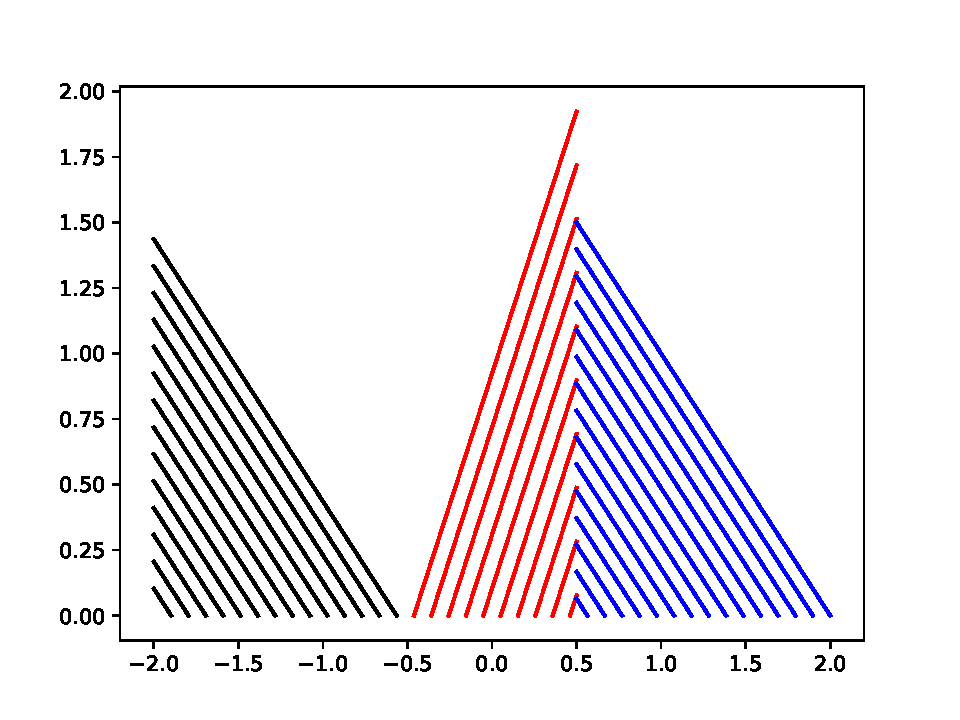
\includegraphics[width=.8\textwidth]{prob2_plot.pdf}
    \caption{Plot of characteristics ($t \le t_b$)}
    \label{fig:prob2_plot}
\end{figure}



\section{Solve the scalar conservation law with subsequent IC}
\begin{gather*}
    \ppt{u} + \pp{}{x}\left(\frac{e^u}{2}\right) = 0\\
    u(x,0) = \begin{cases}
        2, & -1 < x < 1\\
        0, & \text{otherwise}
        \end{cases}
\end{gather*}

We begin to solve this problem by determining which type of discontinuity we
have present in the initial condition. We notice that the IC produces values of
$u$ such that at $x = 1$ we have a shock wave, and at $x = -1$ we have a
rarefraction wave. Thus we determine the solution by identifying the shock speed
$s$ and filling in the rarefraction wave. In order to do so we first resolve the
shock. 

\begin{gather*}
    F(u) = F'(u) = \frac{1}{2}e^{u}\\
    s = \frac{F(2) - F(0)}{2 - 0} \approx \frac{3.19}{2} = 1.595
\end{gather*}

We find that the shock propagates with a speed in the x-t plane of 1.595. Note
that with this information we can find the time $t_b$ in which the shock front
intersects with the tail of the rarefraction wave. We have that the shock front
and the right most tail of the rarefraction wave are separated by $\Delta x =
2$. The right tail of the shock has a speed of $c \approx 3.69$. Therefore, we
have,
\begin{gather*}
    3.69t_b = 1.595t_b + 2\\
    t_b = \frac{2}{2.095} \approx 0.954
\end{gather*}

In order to fill in the rarefraction wave, we adjust the initial condition to be
continuous near the discontinuity at $x = -1$. We have,

\begin{gather*}
    x = \begin{cases}
        \frac{t}{2} + s & \text{if } s + 1 \le -\epsilon\\
        \frac{te^{s/\epsilon + 1}}{2} - 1 & \text{if } -\epsilon <  s + 1 < \epsilon\\
        \frac{te^2}{2} + s & \text{if } s + 1 \ge \epsilon
        \end{cases}
\end{gather*}
We can then complete the inverse mapping, 
\begin{gather*}
    s = \begin{cases}
        x - \frac{t}{2} & \text{if } x \le \frac{t}{2} - 1 \\
        \epsilon \left(\ln\left(\frac{2(x-1)}{t}\right) + 1\right) & \text{if } \frac{t}{2} - 1 < x < \frac{te^2}{2} -1\\
        x - \frac{te^2}{2} & \text{if } x \ge  \frac{te^2}{2} -1 
    \end{cases}
\end{gather*}



\section{Weak solutions of the conservation laws}

\section{Review on WENO and Numerical Methodology (no response required)}

\end{document}
